%% Copernicus Publications Manuscript Preparation Template for LaTeX Submissions
%% ---------------------------------
%% This template should be used for copernicus.cls
%% The class file and some style files are bundled in the Copernicus Latex Package, which can be downloaded from the different journal webpages.
%% For further assistance please contact Copernicus Publications at: production@copernicus.org
%% https://publications.copernicus.org/for_authors/manuscript_preparation.html


%% Please use the following documentclass and journal abbreviations for preprints and final revised papers.

%% 2-column papers and preprints
\documentclass[tc, manuscript]{copernicus}
\usepackage{amsmath}


%% Journal abbreviations (please use the same for preprints and final revised papers)


% Advances in Geosciences (adgeo)
% Advances in Radio Science (ars)
% Advances in Science and Research (asr)
% Advances in Statistical Climatology, Meteorology and Oceanography (ascmo)
% Annales Geophysicae (angeo)
% Archives Animal Breeding (aab)
% ASTRA Proceedings (ap)
% Atmospheric Chemistry and Physics (acp)
% Atmospheric Measurement Techniques (amt)
% Biogeosciences (bg)
% Climate of the Past (cp)
% DEUQUA Special Publications (deuquasp)
% Drinking Water Engineering and Science (dwes)
% Earth Surface Dynamics (esurf)
% Earth System Dynamics (esd)
% Earth System Science Data (essd)
% E&G Quaternary Science Journal (egqsj)
% European Journal of Mineralogy (ejm)
% Fossil Record (fr)
% Geochronology (gchron)
% Geographica Helvetica (gh)
% Geoscience Communication (gc)
% Geoscientific Instrumentation, Methods and Data Systems (gi)
% Geoscientific Model Development (gmd)
% History of Geo- and Space Sciences (hgss)
% Hydrology and Earth System Sciences (hess)
% Journal of Bone and Joint Infection (jbji)
% Journal of Micropalaeontology (jm)
% Journal of Sensors and Sensor Systems (jsss)
% Magnetic Resonance (mr)
% Mechanical Sciences (ms)
% Natural Hazards and Earth System Sciences (nhess)
% Nonlinear Processes in Geophysics (npg)
% Ocean Science (os)
% Polarforschung - Journal of the German Society for Polar Research (polf)
% Primate Biology (pb)
% Proceedings of the International Association of Hydrological Sciences (piahs)
% Scientific Drilling (sd)
% SOIL (soil)
% Solid Earth (se)
% The Cryosphere (tc)
% Weather and Climate Dynamics (wcd)
% Web Ecology (we)
% Wind Energy Science (wes)


%% \usepackage commands included in the copernicus.cls:
%\usepackage[german, english]{babel}
%\usepackage{tabularx}
%\usepackage{cancel}
%\usepackage{multirow}
%\usepackage{supertabular}
%\usepackage{algorithmic}
%\usepackage{algorithm}
%\usepackage{amsthm}
%\usepackage{float}
%\usepackage{subfig}
%\usepackage{rotating}


\begin{document}

\title{Solid earth modulation of marine outlet glacier response}


% \Author[affil]{given_name}{surname}

\Author[1]{Andrew}{Hoffman}
%\Author[1]{Jessica}{Badgeley}
%\Author[2]{Katie}{Brennen}
%\Author[3]{John}{Christian}
%\Author[4]{Natalya}{Gomez}
%\Author[1]{Gerard}{Roe}

\affil[1]{Department of Earth and Space Sciences, University of Washington, Seattle, Washington, USA}

%\affil[2]{Department of Atmospheric Sciences, University of Washington, Seattle, Washington, USA}

%\affil[3]{School of Earth and Atmospheric Sciences, Georgia Institute of Technology, Atlanta, Georgia, USA }

%\affil[4]{Department of Earth and Planetary Sciences, McGill University, Montreal, Quebec, Canada }


%% The [] brackets identify the author with the corresponding affiliation. 1, 2, 3, etc. should be inserted.

%% If an author is deceased, please mark the respective author name(s) with a dagger, e.g. "\Author[2,$\dag$]{Anton}{Smith}", and add a further "\affil[$\dag$]{deceased, 1 July 2019}".

%% If authors contributed equally, please mark the respective author names with an asterisk, e.g. "\Author[2,*]{Anton}{Smith}" and "\Author[3,*]{Bradley}{Miller}" and add a further affiliation: "\affil[*]{These authors contributed equally to this work.}".


\correspondence{hoffmaao@uw.edu}

\runningtitle{Solid earth modulation of marine outlet glacier response}

\runningauthor{Hoffman et al.}





\received{}
\pubdiscuss{} %% only important for two-stage journals
\revised{}
\accepted{}
\published{}

%% These dates will be inserted by Copernicus Publications during the typesetting process.


\firstpage{1}

\maketitle



\begin{abstract}
The dynamics of marine-terminating outlet glaciers and the solid earth are of fundamental interest in glaciology.
In this study, we analyze the response of a coupled marine outlet glacier-bedrock system to different sources of climate forcing.
We find that isostacy fundamentally changes the response of marine outlet glacier systems to surface-mass-balance forcing applied over the interior and the oceanic forcing applied at the grounding line.
The reduced model is shown to emulate the behavior of more complex numerical models of ice flow.
Together, these models demonstrate that ocean forcing first engages the fast, local response, and then the slow adjustment of interior ice, whereas surface-mass-balance forcing is dominated by the slow interior adjustment.
We also demonstrate the importance of the timescales of stochastic forcing for assessing the natural variability of outlet glaciers, highlighting that decadal persistence in ocean variability can affect the behavior of outlet glaciers on centennial and longer timescales.
Finally, we show that these transient responses have important implications for: attributing observed glacier changes to natural or anthropogenic influences; the future change already committed by past forcing; and the impact of past climate changes on the preindustrial glacier state, against which current and future anthropogenic influences are assessed.
\end{abstract}



\section{Introduction} 
Ice-sheet mass change in Antarctica and Greenland is primarily controlled by two processes: thinning at the marine ice-sheet margin due to ocean melt and consequent grounding line position change, and changes in accumulation and surface melt in the ice-sheet interior. 
These mass change mechanisms affect the configuration of the ice sheet differently, eliciting different ice-sheet responses. 
Ocean melt forcing tends to evoke a rapid (multi-decadal) response in glacier length that drives inland thinning from the margin while surface mass balance forcing drives a slow (multi-century) response integrated over the time it takes for the glacier to convey the surface mass balance anomaly to the grounding line (Christian et al 2020, Robel et al 2018).
These response times carry significance for the temporal controls on glacier behavior and can be related to properties of the conveying ice-stream like the glacier geometry, the mechanisms that govern glacier sliding, and the forcing variability.
Marine ice-sheet response times also overlap with the characteristic viscoelastic response time of the solid earth.
The interplay between the deforming geoid due to ice loading and unloading and glacier mass change has been well studied (i.e Weertman 1972; Weertman 1980b; Pollard et al. 1984) and tangentially linked to the stability of geometrically vulnerable marine outlet glaciers through local sea-level adjustment (Gomez et al 2010). 
Understanding the past and future contribution of ice-sheet mass change to distributed sea-level change has motivated acquisition of geodetic time series and coupled simulation of the earth, ice-sheet, sea-level system. 
Together, observations and fully coupled global models have helped quantify committed spatial patterns of sea-level change and the imprinted signature of past ice-sheet configurations in paleo sea-level markers; however, fundamental questions remain regarding the coupled influence of forcing variability, and the natural frequencies of the solid-earth system on ice-sheet response.

Here we combine a simple kinematic description of a marine ice-sheet with a simplified model of the lithosphere to understand the response spectra of glacier volume and length change due to isostasy. 
Our approach is to conduct idealized model experiments that isolate key physical principles of coupled glacier solid-earth system in response to climate variability. 
We follow Robel et al (2018), and Christian et al. (2020) and focus exclusively on stable prograde geometries where the reduced model yields simple physical and mathematical interpretations of a more complicated numerical model’s response to forcing.

We first review the problem and use a dynamical model to understand the filtering properties of a simple marine terminating outlet glacier-bedrock coupled system. We then build on simple kinematic models of marine outlet glacier dynamics, adding a glacier isostatic adjustment (GIA) stage and linearize the kinematic system of equations to understand the projection of surface mass balance and ocean melt forcing onto the eigenmodes of a model that includes the effects of GIA. 
We then use the modified glacier response spectra and the character of perturbations about stable solutions to understand the relative magnitude of GIA on ice sheet mass change.
We show that the stable outlet glacier coupled to the deflectable lithosphere resonates at a frequency that depends on the response time of the asthenosphere as well as the geometry, rheology and sliding properties of the glacier.

\section{Simple ice-sheet-bedrock model and response to ocean and interior forcing}

Before describing the models we use to understand coupled ice-sheet-bedrock response to external forcing, it is useful to begin by describing the geometry and basic flux arguments of the system we are investigating. We consider an idealized stable outlet glacier resting on continental lithosphere, a schematic of which is presented in figure 1a. Ice enters as snow accumulates over the interior and flows from the interior towards the ocean on a prograde bed, exiting the system where it reaches floatation at the grounding zone. Beyond this point, floating ice is assumed to calve or melt due to contact with the ocean. The ice sheet rests on the lithosphere, which we assume to be in floating equilibrium with the underlying heavier substrate in the asthenosphere. As the ice volume changes as the glacier grows or shrinks, the continental lithosphere bends such that the total mass of the ice-sheet-lithosphere-asthenosphere column remains constant. The deflection of the lithosphere follows immediately from the evolving geometry of the ice sheet, and the ratio of the overlying fluid density (water or ice), to that of the substratum. In equilibrium, the output ice-flux of the coupled glacier-bedrock system ($Q_g$) equals the surface mass balance integrated over the glacier catchment and the glacier and bedrock geometry do not change.

\subsection{Flow-line model}
To simulate the dynamics of a coupled outlet-glacier bedrock system, we begin with a 1-D (flowline) version of the ice-sheet-bedrock model developed by Pollard and Deconto (2012). The evolution of local ice thickness at each grid node reflects the balance of mass exchange at the surface and horizontal ice-flux divergence: 
\begin{equation}
\frac{\partial h}{\partial t} = S - \frac{\partial \bar{u}h}{\partial x},
\end{equation}
where $S$ is the local surface mass balance and $\bar{u}$ is the depth-averaged horizontal ice velocity. The velocity profiles have contributions from longitudinal stretching, shear, and basal sliding.

See table 1 for descriptions of each parameter. 
Response time series of glacier length, thickness and the bedrock slope are shown in figure 2 forced with the same white noise surface mass balance used in the initial example.

Bedrock elevation changes with ice and ocean loading as a combination of time-lagged asthenosphereic relaxation towards isostatic equilibrium, and modification of the applied load by the elastic lithosphere. The downward deflection $w_b$ of the fully relaxed response is given by 
\begin{equation}
D\nabla^4 w_b + \rho_b g w_b = q
\end{equation}

where $D = 10^{25} N\cdot m$ is the flexural rigidity of the lithosphere, $\rho_b$ is the bedrock density and $g$ is gravitational acceleration. The applied load is 
\begin{equation}
q = \rho_i g h + \rho_w g h_w - \rho_i g h_i^{eq} - \rho_w g h_w^{eq} 
\end{equation}

where $h$ is ice thickness, $h_w$ is ocean column thickness and $h^{eq}$ and $h_w^eq$ are their values in the equilibrium state. The deflection is summed over indiviual point loads of all grid cells, and assumed to be proportional to the unbalanced pressure at the top of the asthenosphere. The actual bedrock rate of change is given by:
\begin{equation}
\frac{\partial h_b}{\partial t} = -\frac{1}{\tau} \left(h_b - h_b^{eq} + w_b \right)
\end{equation}
where $h_b$ is the current bedrock elevation, $h_b^{eq}$ is its equilibrium value and $\tau$ is the $\approx 3000yr$ asthenosphere relaxation timescale.

\subsection{kinematic model}

Ice-sheet mass change can be described in two stages for an idealized stable ice-sheet (Robel et al 2018; Christian et al 2020).
In the first stage, accumulation falls in the interior and flows under its own weight towards the outlet glacier margins.
The surface mass balance flux ($L\cdot S$) is modified by the interior flux ($Q$) according to the partitioning of stress accommodated by internal deformation and basal traction.
The interior reservoir of the ice-sheet drains according to this interior flux until it reaches the second stage where stresses change as the glacier goes afloat giving rise to a kinematic grounding line flux $Q_g$, that depends nonlinearly on the grounding zone ice thickness, $h_g$,
\begin{align}
Q_g=\Omega h_g^\beta.
\end{align}
 Two coupled equations capture the response of $H$, the interior thickness, and $L$, the glacier length, as they relax towards a steady state that balances all three fluxes:
 \begin{align}
\frac{dH}{dt} &=S - \frac{Q}{L}-\frac{H}{h_g L}(Q-Q_g)&\\
\frac{dL}{dt} &=\frac{1}{hg}(Q-Q_g).&
\end{align}
Descriptions of the kinematic fluxes ($L\cdot S, Q, Q_g$) with time series of forcing (i.e. surface mass balance, $S$ and ocean melt rate, $\Omega$) form a closed system of ordinary differential equations that describe variations in glacier thickness and length.
To review the behavior of this coupled two-stage system and introduce the parameters that describe glacier response, we use variations of the equilibrium two-stage ice-steam geometry described by Christian et al. (2020; Figure 1).
The domain begins at an ice divide and thus has a zero-flux boundary condition.
The surface mass balance is $0.5 m a^{-1}$ ice equivalent and is assumed to be spatially uniform across the interior.
The glacier has an equilibrium length of $\approx185km$, a maximum thickness of $\approx1410m$, and a grounding line thickness of $\approx 526m$, which are generally representative of Greenland outlet glaciers and paleo-ice sheets of North America.
The bed elevation at the ice divide is $-100m$, and the equilibrium slope is $2m/km$. 

\begin{figure}[t]
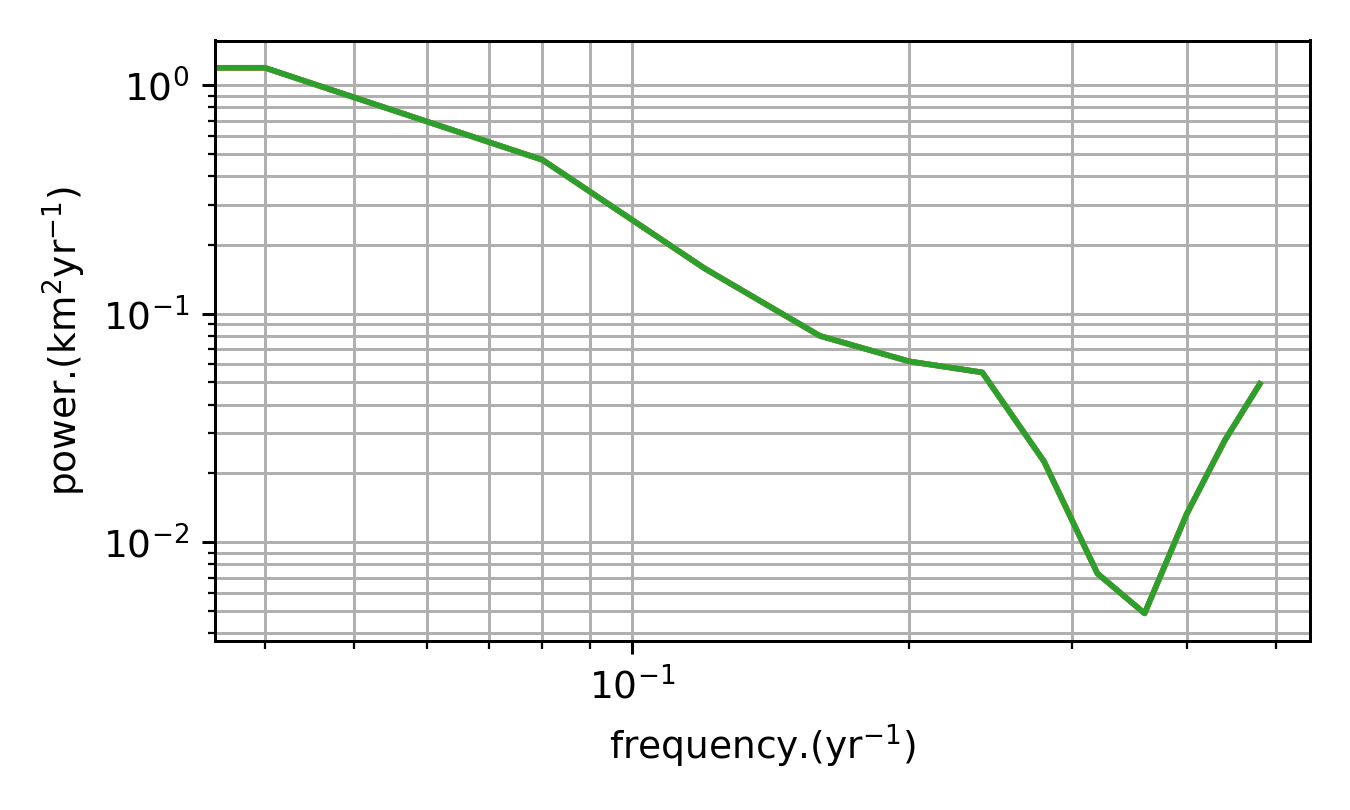
\includegraphics[width=8.3cm]{../figures/simulation0203.png}
\caption{(a) Model schematic and response to forcing..}
\end{figure}


To demonstrate the glaciological sensitivity of the filtering properties of the two stage model, we adopt two parameterizations of the interior flux, $Q$, and grounding zone flux, $Q_g$ associated with a glacier sliding over hard bedrock (form-drag friction relation), and a glacier sliding over deformable sediment (coulomb friction relation). These two parameterizations do not bound the behavior of glacier response (), but give some sense of glaciological parameter sensitivity to applied forcing that can compare with simulations with an additional bedrock deflection stage.

Using synthetic time series of white noise ocean melt and surface mass balance anomalies with variance equal to $10\%$ of the equilibrium interior surface mass balance flux and equilibrium ocean flux, we force glaciers parameterized with different flux criteria normalized to have the same equilibrium geometry and analyze their length change spectra (figure 2).
In these simulations the bedrock topography is fixed, and the response spectra can be described using spectral power laws that represent the physical processes that result from nonlinear energy transfer between the applied forcing and the mechanics of sliding and ice flow.
The spectra capture the ice sheet’s capacity to filter different frequencies of forcing and demonstrate the glaciological sensitivity of the glacier-bedrock system to the grounding zone flux parameterization.
In agreement with Schoof et al (2007) and Tsai et al (2015), the regularized coulomb friction glacier is more sensitive to ocean melt variability than the hard-bedded glacier. 

From these grounding zone flux conditions, we see principal glaciological controls change the responsiveness of the two-stage marine ice sheet to perturbations in the surface mass balance and ocean mass balance forcing by changing the intrinsic properties of the glacier filter

Figure 2. The response function of the marine glacier forced with the same white noise variability in surface mass balance for the grounding line flux assuming different relationships between sliding speed and basal shear stress are shown in figure 2.



\begin{figure}[t]
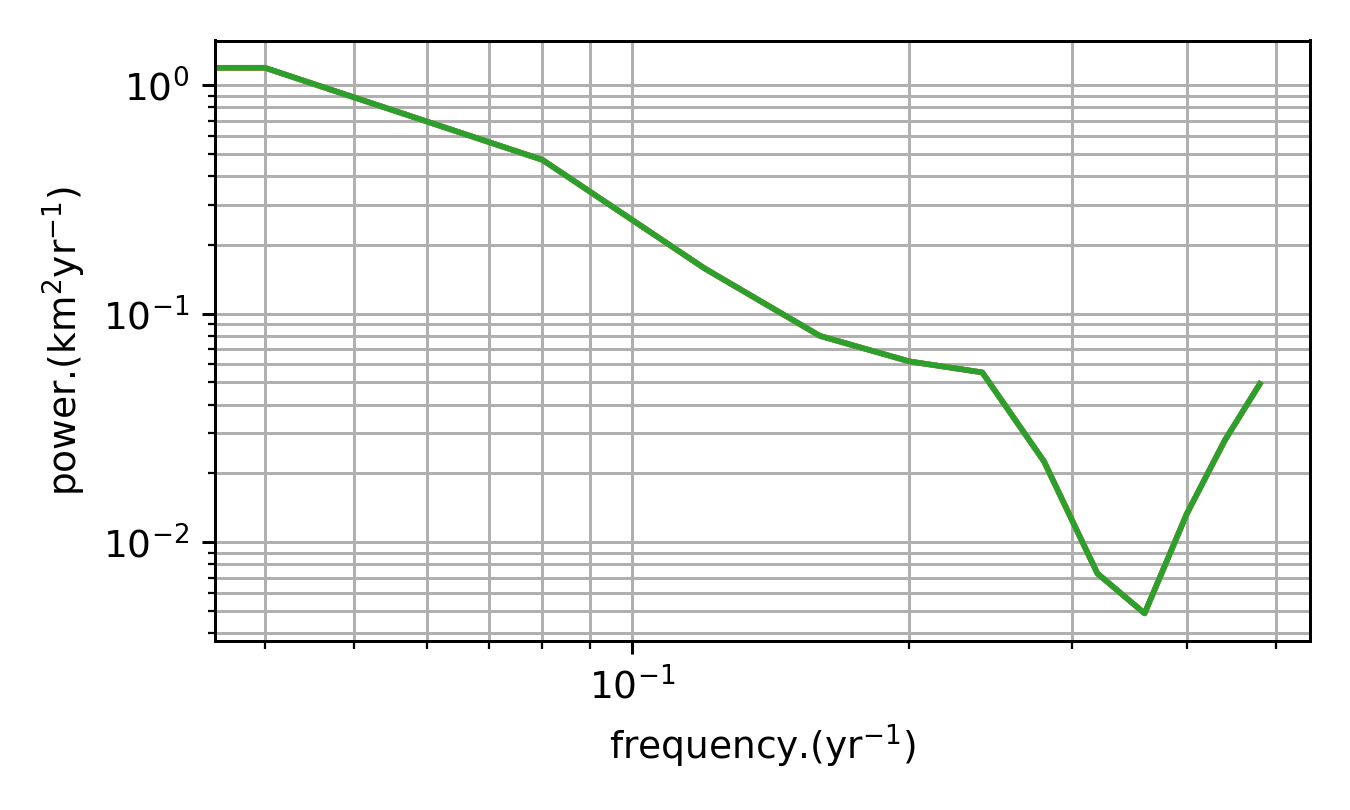
\includegraphics[width=8.3cm]{../figures/simulation0203.png}
\caption{(a) Glacier length and thickness change for a regularized coloumb and hard-bedded outlet glacier system. (b) Power spectral density for each glacier as a function of frequency calculated via Welch's method with a window of $1/16$ the total time series ($10^6$ years).}
\end{figure}



\begin{table}[h]
    \begin{tabular}{l|l}
        Symbol & Meaning \\
        \hline
        $L$ & glacier length \\
        $H$ & interior thickness \\
        $b_x$ & bedrock slope \\
        $h_g$ & grounding zone thickness \\
        $Q$ & interior flux \\
        $Q_g$ & grounding zone flux \\
        $b_{x_0}$ & equilibrium bedrock slope \\
        $\tau$ & response time of solid earth  \\
    \end{tabular}
    \caption{Mathematical symbols}
\end{table}


\section{A simple model for the coupled solid-earth outlet-glacier system}

The simplest model for bedrock adjustment is based on the principle of local isostatic equilibrium. The lithosphere is assumed to be in floating equilibrium with the underlying heavier substrate in the asthenosphere, and the total mass of a vertical column is constant.
When an ice sheet is present, the lithosphere bends downward, replacing part of the heavier material in the asthenosphere, such that the total mass of the column is constant. The deflection follows immediately from the ice geometry defined by the ice thickness $H$, glacier length $L$, and the ratio of the overburden fluid density (ice, or water) to that of the substratum.
The adjustment in bedrock slope deflection is modulated by the viscous flow of the asthenosphere, which has a characteristic response time, $\tau$.
This change in bedrock slope defines the new bed geometry and grounding line position, introducing a third stage to the outlet glacier model.
The new system of equations that define the glacier-bedrock system are: 
		

\begin{align}
    \frac{dL}{dt} & = \frac{1}{h_g(L,b_x)}\cdot(Q(L,H)-Q_g(L,b_x)), \\
    \frac{dH}{dt} & = S-\frac{Q_g(L,b_x)}{L}-\frac{H}{h_g(L,b_x) L} \cdot (Q(L,H)-Q_g(L,b_x)), \\
    \frac{db_x}{dt} & = -\frac{1}{\tau}(b_x - b_{x_0}).
\end{align}



\subsection{Projection of variability on system eigenmodes}
The outlet glacier model equations (2-4)  can be linearized to understand changes in the glacier length, thickness, and bedrock slope about a local equilibrium position $\bar{L}, \bar{H}$, and $\bar{m}$. At this stable equilibrium, the interior and grounding zone fluxes balance one another and the evolution of fluctuations about the average length, thickness and slope can be written as

\begin{align}
\frac{\partial}{\partial t}\bf{Y} &= \bf{JY}+\bf{S} \it{f(t)}& \\
\frac{\partial}{\partial t}
 \begin{bmatrix} L' \\ H' \\ b_x' \end{bmatrix}
 &=
  \begin{bmatrix}
   A_L & A_H & A_{b_x}  \\
   B_L & B_H& B_{b_x} \\
   C_L & C_H & C_{b_x}
   \end{bmatrix}
    \begin{bmatrix} L' \\ H' \\ b_x' \end{bmatrix}
    +
    \begin{bmatrix} \bar{h_g}^{-1} \\ \bar{L}^{-1}\left(\frac{\bar{H}}{\bar{h_g}}-1\right) \\ 0 \end{bmatrix} Q_g'
    + 
    \begin{bmatrix} 0 \\ 1 \\ 0 \end{bmatrix} S'&
\end{align}

where $A_H, A_L, A_m, B_H, B_L, B_m, C_H, C_L,$ and $C_m$ describe the couplings between length, thickness, and bed-slope changes (Christian et al 2020; see appendix for coefficient solutions), and $Q_g'$ and $S'$ describe the projection of terminus and interior climate forcing on each state variable. The coupling described by each coefficient is significantly more complex because of the additional feedback with the bedrock slope, so we substitute representative glacier geometry, rheology and sliding parameter values into the vectorized system of equations to understand the solution character empirically. The parameters used are shown in table 2.

\begin{table}[h]
    \begin{tabular}{l|l}
        \hline
        \bf{parameter} & \bf{value} \\
        \hline
        equilibrium length, $\bar{L}$ ($km$) &  182 \\
        equilibrium thickness, $\bar{H}$ ($m$) & 1412 \\
        equilibrium slope, $\bar{b_x}$ ($m/km$) &  -2  \\
        sliding exponent, $m$ & 1/3 \\
        sliding coefficient $C$ ($Pa\cdot m^{-1/3}s^{1/3}$) & 7624000 \\
        deformation exponent, $n$ & 3 \\
        seawater density, $\rho_w$ ($kg \cdot m^{-3}$)  & 1028 \\
        ice density, $\rho_i$ ($kg \cdot m^{-3}$) & 917 \\
        bed elevation at divide, $b_0$ ($m$) & -100 \\
        $\beta$ & 19/3 \\
        $\gamma$ & 3 \\
        $\tau$ ($yr$) & 3000\\
    \end{tabular}
    \caption{Mathematical symbols}
\end{table}



With the addition of the third-stage wherein the bedrock slope is allowed to respond with length and thickness change, we find that the solutions for linearized glacier-bedrock model become complex. We project the vector-form equation for the system on to the system eigenmodes, which can be written as simple one-dimensional linear ordinary differential equations for which we can write the green's function in the time domain, the power spectral density, and the covariance function explicitly to further understand the character of the response. 

\begin{align}
\frac{d}{dt} m_s  &=& -\alpha_s m_s + \sigma_s f(t)\\
\frac{d}{dt} m_f &=& -\alpha_f m_f + \sigma_s f(t)\\
\frac{d}{dt} m_{i} &=& -\alpha_i m_{i} + \sigma_{i} f(t)
\end{align}


\begin{figure}[t]
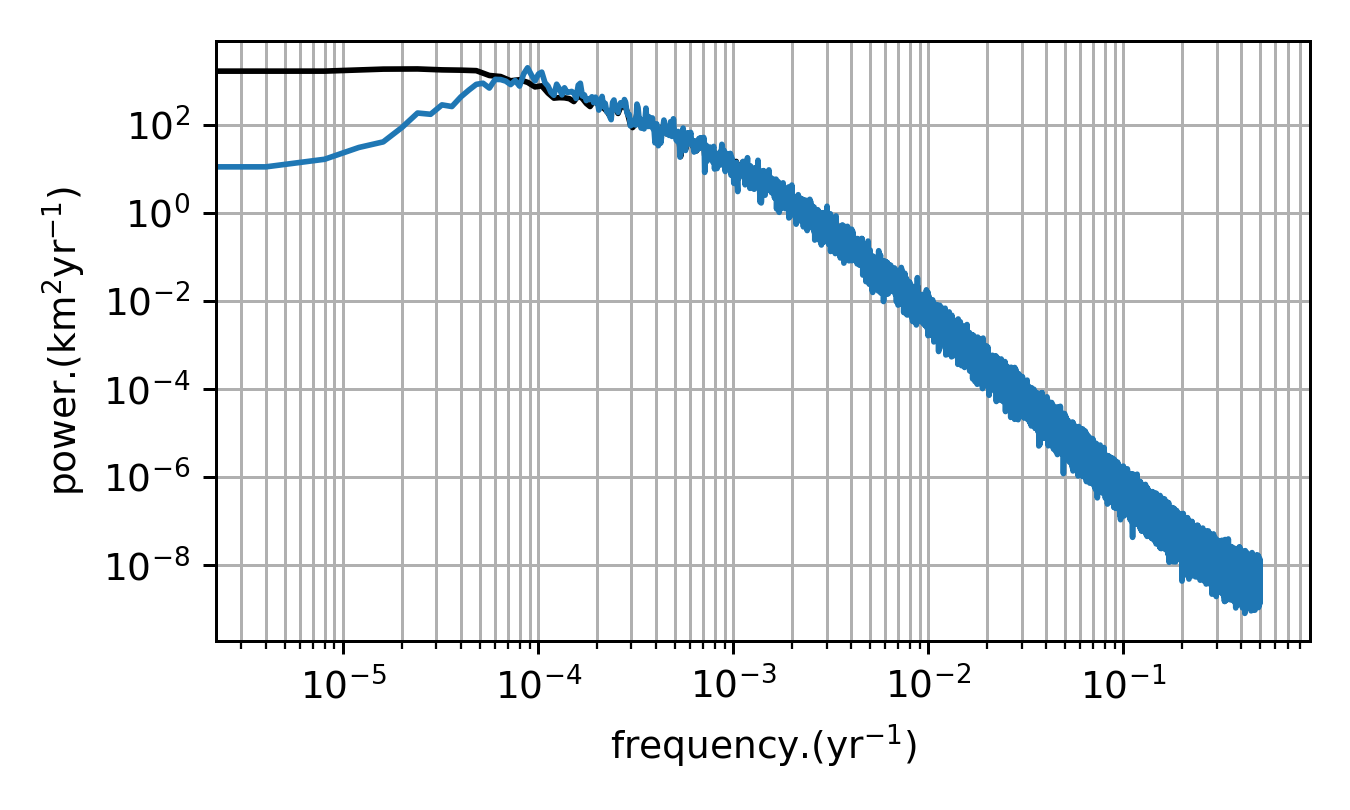
\includegraphics[width=8.3cm]{../figures/simulationSMB03.png}
\caption{Model response from theoretical eigenmode decomposition.
The left column is the response to precipitaion forcing ($\Delta S = −0.2$). 
The right column is the response to Grounding Line forcing ($\Delta Q_g = 0.2$).
The projections of the eigenmodes onto the $H, L$ are identical. The only difference comes from ($\sigma H, \sigma L$) which affects how much each type of forcing excites the fast and slow eigenmodes.
In particular, we notice that Grounding line forcing excites the fast mode much more strongly than precipitation forcing does.}
\end{figure}


Figures *-* demonstrate that the inclusion of isostatic adjustment significantly changes the response of marine-terminating outlet glaciers. 
In the next section, we examine the consequences of filtering properties of the coupled ice-sheet-bedrock system for three key questions in glaciology: 
How does GIA modify the committed response of marine ice-sheets to forcing?
How does damping at non-resonant frequencies affect the spectra of ice volume variability preserved in proxy records?
And how could the whitening of loe 


\section{Characteristic time scales}
\subsection{Comparison with two-stage model}
Robel et al. (2018) and Christian et al. (2020) showed that the two-stage model emulates the response of different flowline models to interior surface mass-balance anomalies and grounding flux perturbations. 

Figure 2 shows output from the two stage marine outlet glacier model and the model that also includes variations in bedrock slope due to GIA.

\begin{figure}[t]
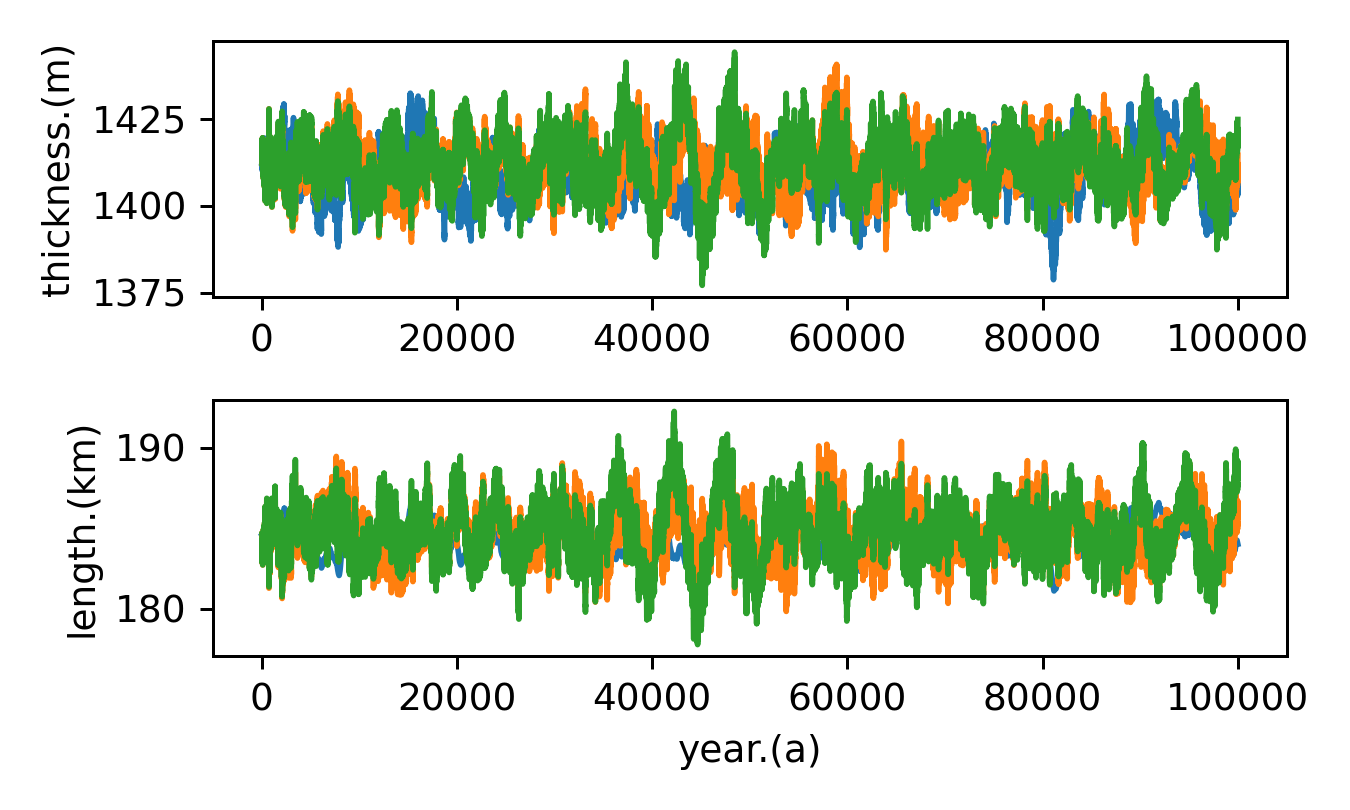
\includegraphics[width=8.3cm]{../figures/simulation0101.png}
\caption{Time series of the glacier length and thickness variations for a simulation with the bedrock geometry fixed, and a simulation with the bedrock slope allowed to vary.}
\end{figure}


\begin{figure}[t]
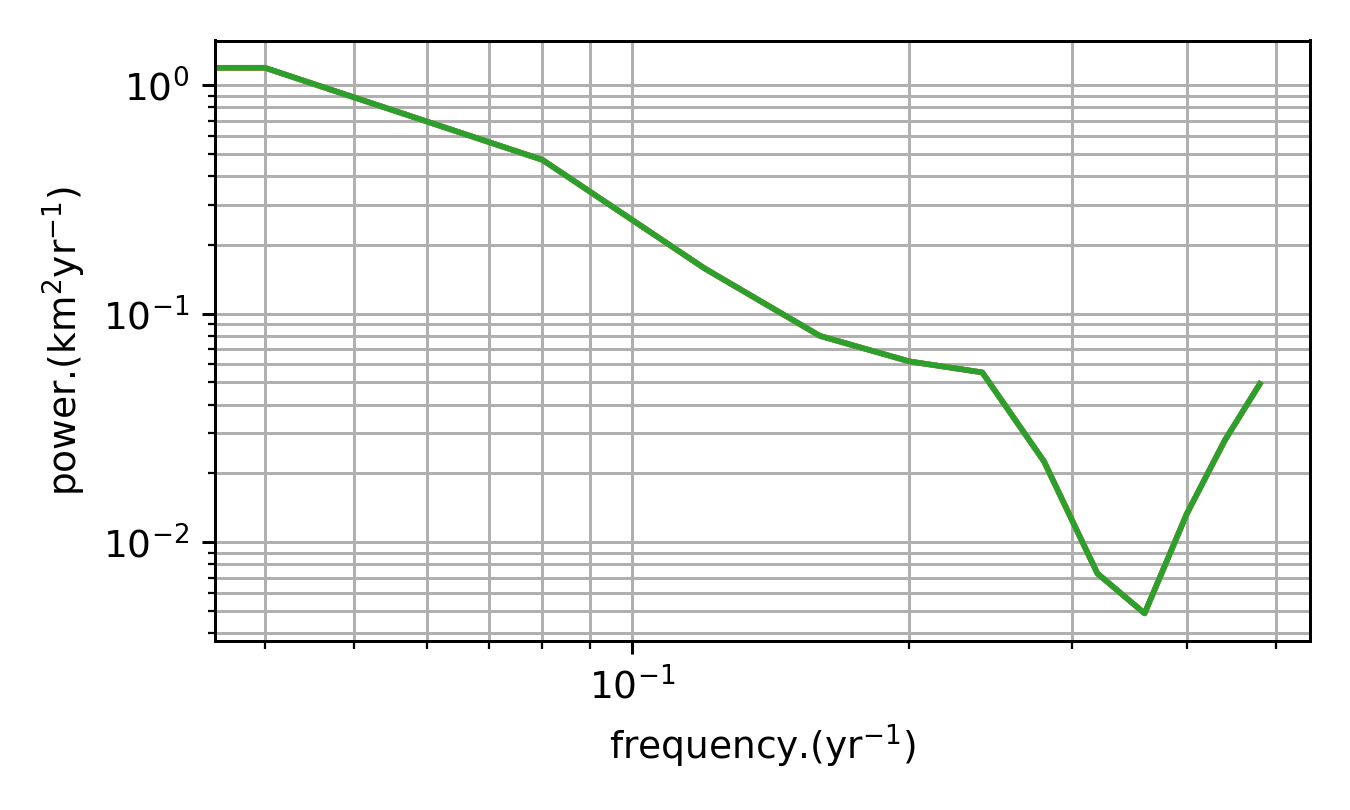
\includegraphics[width=8.3cm]{../figures/simulation0203.png}
\caption{(a) Autocorrleation as a function of time lag. (b) Power spectral density as a function of frequency calculated via Welch's method with a window of $1/16$ the total time series ($10^6$ years).}
\end{figure}

\section{summary and discussion}

\subsection{Climate-bedrock feedback implications}
Any system with a non-zero response time will lag the applied forcing.
Committed change refers to the total response such a system would need to undergo to attain equilibrium with the current level of forcing.
In the previous sections, variability was imposed with a flat power spectra (i.e. white noise); however inertia of the climate system.

\subsection{sea-level}


\conclusions  
Our simple modeling demonstrates a subtle feedback between multi-milenia climate variability and the modulation of marine ice-sheet bedrock that tends to stabilize the marine ice-sheet system by damping low frequency oscillations in glacier thickness and glacier length relative to simulations that assume no bedrock response. 
The same feedback amplifies oscillations in glacier length at the resonant frequency of the bedrock.


%% The following commands are for the statements about the availability of data sets and/or software code corresponding to the manuscript.
%% It is strongly recommended to make use of these sections in case data sets and/or software code have been part of your research the article is based on.

\codedataavailability{The code used to run the simulations included in the text is freely available at https://github.com/hoffmaao/gia2stage (last accessed April 20 2021).} 


%\dataavailability{TEXT} %% use this section when having only data sets available


%\videosupplement{TEXT} %% use this section when having video supplements available


\appendix
\section{Derivation of linear model}    %% Appendix A

\begin{multline*}
    A_L = \frac{-\bar{H}^\alpha \bar{L}^{-1 - \gamma} \gamma \nu - \bar{m} \beta \lambda \Omega((b_0 + \bar{L} \bar{m}) \lambda)^{-1 + \beta}}{(b_0 +\bar{L} \bar{m}) \lambda} + \frac{(\bar{m} (\bar{H}^\alpha \bar{L}^-\gamma \nu + \Omega(b_0 + \bar{L} \bar{m}) \lambda)^\beta}{(b_0+ \bar{L} \bar{m})^2 \lambda}, \\
    A_H =  \frac{- \bar{H}^{-1 + \alpha} \bar{L}^-\gamma \alpha \nu}{(b_0 + \bar{L} \bar{m}) \lambda}, \\
    A_m =  \frac{-((\bar{L} \beta (-(b_0 + \bar{L} \bar{m}) \lambda)^{-1 + \beta} \Omega)}{b_0 + \bar{L} \bar{m}} + \frac{(\bar{L} (\bar{H}^\alpha \bar{L}^-\gamma \nu - (-(b_0 + \bar{L} \bar{m}) \lambda)^\beta \Omega))}{(b_0 + \bar{L} \bar{m})^2 \lambda}, \\
    B_L = \frac{\bar{m} \beta \lambda (-(b_0 + \bar{L} \bar{m}) \lambda)^{-1 + \beta} \Omega)}{\bar{L}} + \frac{((-(b_0 + \bar{L} \bar{m}) \lambda)^\beta \Omega)}{\bar{L}^2} + \frac{(\bar{H} (-\bar{H}^\alpha \bar{L}^(-1 - \gamma) \gamma \nu + \bar{m} \beta \lambda (-(b_0 + \bar{L} \bar{m}) \lambda)^(-1 + \beta) \Omega))}{\bar{L} (b_0 + \bar{L} \bar{m}) \lambda} \\
    - \frac{(\bar{H} \bar{m} (\bar{H}^\alpha \bar{L}^-\gamma \nu - (-(b_0 + \bar{L} \bar{m}) \lambda)^\beta \Omega))}{\bar{L} (b_0 + \bar{L} \bar{m})^2 \lambda} - \frac{(\bar{H} (\bar{H}^\alpha \bar{L}^-\gamma \nu - (-(b_0 + \bar{L} \bar{m}) \lambda)^\beta] \Omega))}{\bar{L}^2 (b_0 + \bar{L} \bar{m}) \lambda}, \\
    B_H = \frac{\bar{H}^\alpha \bar{L}^(-1 - \gamma) \alpha \nu}{(b_0 + \bar{L} \bar{m}) \lambda} + \frac{\bar{H}^\alpha \bar{L}^-\gamma \nu - (-(b_0 + \bar{L} \bar{m}) \lambda)^\beta \Omega}{\bar{L} (b_0 +\bar{ L} \bar{m}) \lambda}, \\
    B_m = \frac{\bar{H} \beta (-(b_0 + \bar{L} \bar{m}) \lambda)^{-1 + \beta} \Omega}{b_0 + \bar{L} \bar{m}} + \beta \lambda (-(b_0 + \bar{L} \bar{m}) \lambda)^{-1 + \beta} \Omega - \frac{\bar{H} (\bar{H}^\alpha \bar{L}^-\gamma \nu - (-(b_0 + \bar{L} \bar{m}) \lambda)^\beta \Omega)}{(b_0 + \bar{L} \bar{m})^2 \lambda}, \\
    C_L =-\frac{-\frac{1}{3} \bar{L} \bar{m} \kappa - 
  \frac{1}{3} (-b_0 + 2\bar{H} + \bar{L} \bar{m}) \kappa}{\tau}, \\
    C_H=\frac{2 \bar{L} \kappa}{3 \tau}, \\
    C_m=-\frac{1 - \frac{(\bar{L}^2 \kappa)}{3}}{\tau}. \\
\end{multline*}
     
\subsection{}     %% Appendix A1, A2, etc.


\noappendix       %% use this to mark the end of the appendix section. Otherwise the figures might be numbered incorrectly (e.g. 10 instead of 1).

%% Regarding figures and tables in appendices, the following two options are possible depending on your general handling of figures and tables in the manuscript environment:

%% Option 1: If you sorted all figures and tables into the sections of the text, please also sort the appendix figures and appendix tables into the respective appendix sections.
%% They will be correctly named automatically.

%% Option 2: If you put all figures after the reference list, please insert appendix tables and figures after the normal tables and figures.
%% To rename them correctly to A1, A2, etc., please add the following commands in front of them:

\appendixfigures  %% needs to be added in front of appendix figures

\appendixtables   %% needs to be added in front of appendix tables

%% Please add \clearpage between each table and/or figure. Further guidelines on figures and tables can be found below.



\authorcontribution{AOH, JB and KB theorized the study, JEC supported PSUICE flow modeling. RCS identified proxy records and analyzed their spectra. AOH wrote the paper and all authors contributed revisions.} %% this section is mandatory

\begin{acknowledgements}
AOH was supported by NASA FINESST grant progran ()
\end{acknowledgements}




%% REFERENCES

%% The reference list is compiled as follows:

\begin{thebibliography}{}

\bibitem[AUTHOR(YEAR)]{LABEL1}
REFERENCE 1

\bibitem[AUTHOR(YEAR)]{LABEL2}
REFERENCE 2

\end{thebibliography}

%% Since the Copernicus LaTeX package includes the BibTeX style file copernicus.bst,
%% authors experienced with BibTeX only have to include the following two lines:
%%
%% \bibliographystyle{copernicus}
%% \bibliography{example.bib}
%%
%% URLs and DOIs can be entered in your BibTeX file as:
%%
%% URL = {http://www.xyz.org/~jones/idx_g.htm}
%% DOI = {10.5194/xyz}


%% LITERATURE CITATIONS
%%
%% command                        & example result
%% \citet{jones90}|               & Jones et al. (1990)
%% \citep{jones90}|               & (Jones et al., 1990)
%% \citep{jones90,jones93}|       & (Jones et al., 1990, 1993)
%% \citep[p.~32]{jones90}|        & (Jones et al., 1990, p.~32)
%% \citep[e.g.,][]{jones90}|      & (e.g., Jones et al., 1990)
%% \citep[e.g.,][p.~32]{jones90}| & (e.g., Jones et al., 1990, p.~32)
%% \citeauthor{jones90}|          & Jones et al.
%% \citeyear{jones90}|            & 1990



%% FIGURES

%% When figures and tables are placed at the end of the MS (article in one-column style), please add \clearpage
%% between bibliography and first table and/or figure as well as between each table and/or figure.

% The figure files should be labelled correctly with Arabic numerals (e.g. fig01.jpg, fig02.png).


%% ONE-COLUMN FIGURES

%%f
%\begin{figure}[t]
%\includegraphics[width=8.3cm]{FILE NAME}
%\caption{TEXT}
%\end{figure}
%
%%% TWO-COLUMN FIGURES
%
%%f
%\begin{figure*}[t]
%\includegraphics[width=12cm]{FILE NAME}
%\caption{TEXT}
%\end{figure*}
%
%
%%% TABLES
%%%
%%% The different columns must be seperated with a & command and should
%%% end with \\ to identify the column brake.
%
%%% ONE-COLUMN TABLE
%
%%t
%\begin{table}[t]
%\caption{TEXT}
%\begin{tabular}{column = lcr}
%\tophline
%
%\middlehline
%
%\bottomhline
%\end{tabular}
%\belowtable{} % Table Footnotes
%\end{table}
%
%%% TWO-COLUMN TABLE
%
%%t
%\begin{table*}[t]
%\caption{TEXT}
%\begin{tabular}{column = lcr}
%\tophline
%
%\middlehline
%
%\bottomhline
%\end{tabular}
%\belowtable{} % Table Footnotes
%\end{table*}
%
%%% LANDSCAPE TABLE
%
%%t
%\begin{sidewaystable*}[t]
%\caption{TEXT}
%\begin{tabular}{column = lcr}
%\tophline
%
%\middlehline
%
%\bottomhline
%\end{tabular}
%\belowtable{} % Table Footnotes
%\end{sidewaystable*}
%
%
%%% MATHEMATICAL EXPRESSIONS
%
%%% All papers typeset by Copernicus Publications follow the math typesetting regulations
%%% given by the IUPAC Green Book (IUPAC: Quantities, Units and Symbols in Physical Chemistry,
%%% 2nd Edn., Blackwell Science, available at: http://old.iupac.org/publications/books/gbook/green_book_2ed.pdf, 1993).
%%%
%%% Physical quantities/variables are typeset in italic font (t for time, T for Temperature)
%%% Indices which are not defined are typeset in italic font (x, y, z, a, b, c)
%%% Items/objects which are defined are typeset in roman font (Car A, Car B)
%%% Descriptions/specifications which are defined by itself are typeset in roman font (abs, rel, ref, tot, net, ice)
%%% Abbreviations from 2 letters are typeset in roman font (RH, LAI)
%%% Vectors are identified in bold italic font using \vec{x}
%%% Matrices are identified in bold roman font
%%% Multiplication signs are typeset using the LaTeX commands \times (for vector products, grids, and exponential notations) or \cdot
%%% The character * should not be applied as mutliplication sign
%
%
%%% EQUATIONS
%
%%% Single-row equation
%
%\begin{equation}
%
%\end{equation}
%
%%% Multiline equation
%
%\begin{align}
%& 3 + 5 = 8\\
%& 3 + 5 = 8\\
%& 3 + 5 = 8
%\end{align}
%
%
%%% MATRICES
%
%\begin{matrix}
%x & y & z\\
%x & y & z\\
%x & y & z\\
%\end{matrix}
%
%
%%% ALGORITHM
%
%\begin{algorithm}
%\caption{...}
%\label{a1}
%\begin{algorithmic}
%...
%\end{algorithmic}
%\end{algorithm}
%
%
%%% CHEMICAL FORMULAS AND REACTIONS
%
%%% For formulas embedded in the text, please use \chem{}
%
%%% The reaction environment creates labels including the letter R, i.e. (R1), (R2), etc.
%
%\begin{reaction}
%%% \rightarrow should be used for normal (one-way) chemical reactions
%%% \rightleftharpoons should be used for equilibria
%%% \leftrightarrow should be used for resonance structures
%\end{reaction}
%
%
%%% PHYSICAL UNITS
%%%
%%% Please use \unit{} and apply the exponential notation


\end{document}
